\documentclass[10pt,twocolumn,letterpaper]{article}

% --- Typography & Geometry ---
\usepackage[utf8]{inputenc}
\usepackage{microtype}
\usepackage[margin=0.75in,top=0.85in,bottom=0.85in]{geometry}

% --- Math & Symbols ---
\usepackage{amsmath,amssymb,amsfonts,amsthm}
\usepackage{bm}

% --- Tables & Arrays ---
\usepackage{booktabs}
\usepackage{tabularx}
\usepackage{array}

% --- Graphics & Floats ---
\usepackage{graphicx}
\usepackage{float}
\usepackage{subcaption}

% --- Code Listings ---
\usepackage{xcolor}
\usepackage{listings}

\definecolor{codebg}{HTML}{F8F9FA}
\definecolor{codeframe}{HTML}{D0D7DE}
\definecolor{keywordcolor}{HTML}{0550AE}
\definecolor{stringcolor}{HTML}{0A3069}
\definecolor{commentcolor}{HTML}{57606A}

\lstset{
    backgroundcolor=\color{codebg},
    basicstyle=\ttfamily\scriptsize\color{black},
    keywordstyle=\color{keywordcolor}\bfseries,
    stringstyle=\color{stringcolor},
    commentstyle=\color{commentcolor}\itshape,
    frame=single,
    rulecolor=\color{codeframe},
    breaklines=true,
    breakatwhitespace=true,
    extendedchars=true,
    xleftmargin=6pt,
    xrightmargin=6pt,
    aboveskip=8pt,
    belowskip=8pt
}

% --- Hyperlinks ---
\usepackage{hyperref}
\hypersetup{
    colorlinks=true,
    linkcolor=blue!70!black,
    citecolor=blue!70!black,
    urlcolor=blue!70!black
}

% --- Input Title & Authors ---
% Metadata for cosformer
\title{\textbf{Cosformer: Linear Attention with Cosine-Based Positional Reweighting for Pretrained Transformers}}

\author{
  \textbf{Taha Majs}\thanks{Corresponding author: tahamajs@uni.edu} \quad \textbf{Research Team} \\
  Department of Computer Science \\
  Advanced Machine Learning \& Efficiency Laboratory
}

\date{\today}


\begin{document}

\maketitle

% --- Abstract & Keywords Block ---
\begin{abstract}

Softmax attention is the bottleneck of transformer inference for long 
sequences, requiring $\mathcal{O}(L^2)$ time and memory. \textbf{Cosformer} 
(Qin et al., 2022) addresses this by replacing softmax with a non-negative 
kernel (ELU + 1 or softplus) augmented with cosine-based positional 
reweighting, yielding $\mathcal{O}(L)$ attention while preserving locality. 
We present a \textbf{production-hardened port} of Cosformer to pretrained 
transformers, supporting four architecture families -- DistilBERT, 
RoBERTa/BERT, GPT-2, and Qwen/LLaMA -- with exact weight transfer, GQA, 
RoPE, and two distinct computational paths: \textbf{associative accumulation} 
for bidirectional encoders and \textbf{chunked prefix-sum} for causal decoders. 
Base weights are transferred exactly from the pretrained attention; LoRA 
adapters at rank $r = {{LORA_RANK}}$ provide recovery capacity.

We benchmark on SST-2 across three models. Cosformer achieves 
\textbf{{{D\_ACC}}\%} on DistilBERT (baseline {{D\_BASE}}\%, $\Delta$ = {{D\_DELTA}}), 
\textbf{{{R\_ACC}}\%} on RoBERTa ($\Delta$ = {{R\_DELTA}}), and \textbf{{{G\_ACC}}\%} on GPT-2 
($\Delta$ = {{G\_DELTA}}). Inference time is \textbf{{{D\_TIME\_R}}$\times$} baseline on 
DistilBERT and \textbf{{{G\_TIME\_R}}$\times$} on GPT-2. Unlike recent mechanisms that 
collapse on encoders, Cosformer preserves most of the baseline accuracy 
at a modest latency cost. We document the construction of the cosine/sine 
reweighting, the chunked causal scan, and the exact failure modes we 
observed.

\textbf{Keywords:} linear attention, Cosformer, kernel methods, positional 
reweighting, efficient transformers



\vspace{0.5em}
\noindent\textbf{Keywords:} linear attention, Cosformer, kernel methods, positional
\end{abstract}

\vspace{1em}

% --- Paper Body ---
\section{01 Intro}

Draft content for cosformer.


\section{Related Work}

\subsection{Linear Attention}

\textbf{Linear Transformer} (Katharopoulos et al., 2020). Uses $\phi(x) = \text{elu}(x) + 1$ 
without positional reweighting. First to show $\mathcal{O}(L)$ attention 
with reasonable performance.

\textbf{Performer} (Choromanski et al., 2021). Uses random Fourier features 
(RFF) for kernel approximation with theoretical guarantees.

\textbf{Nystr mformer} (Xiong et al., 2021). Uses Nystr m landmarks for low-rank 
attention approximation.

\subsection{Positional Reweighting}

\textbf{Cosformer} (Qin et al., 2022). The direct inspiration for this work. 
Uses cosine/sine reweighting to preserve locality.

\textbf{RoPE} (Su et al., 2021). Rotary position embeddings, standard in modern 
decoders. Not the same as Cosformer's reweighting -- RoPE rotates features, 
Cosformer scales them.

\textbf{ALiBi} (Press et al., 2022). Linear bias on attention scores. Preserves 
locality.

\subsection{Causal Linear Attention}

For causal models, naive linear attention is not enough -- the denominator 
must accumulate causally. Two main approaches:

\textbf{Cumulative sum (cumsum).} Compute running sums over the sequence. 
$\mathcal{O}(L)$ memory, single kernel.

\textbf{Chunked prefix-sum.} Split sequence into chunks; compute intra-chunk 
contributions directly, inter-chunk via state. Used in Cosformer, DeltaNet, 
and others.

\subsection{Pretrained Weight Transfer}

\textbf{DistilBERT} (Sanh et al., 2019). Distillation with weight transfer.

\textbf{LoRA} (Hu et al., 2021). Preserves pretrained weights, adds low-rank 
adapters.

\textbf{Our approach.} Combines exact weight transfer (Q/K/V/O) with LoRA recovery.

\subsection{Position of Our Work}

\begin{table}[H]
\centering
\small
\begin{tabular}{lll}
\toprule
\textbf{Axis} & \textbf{Prior work} & \textbf{Ours} \\
\midrule
\textbf{Method} & Cosformer (published) & Port to pretrained \\
\textbf{Weight transfer} & Rare & Exact, four architectures \\
\textbf{Bidirectional} & Sometimes & Dedicated path \\
\textbf{RoPE support} & Limited & Full support \\
\textbf{Recovery} & From scratch & LoRA \\
\bottomrule
\end{tabular}
\end{table}

\textbf{Key distinction.} Unlike most linear-attention papers that train from 
scratch, we focus on \textbf{weight-preserving port} to pretrained models. This 
requires careful handling of the \texttt{copy\_weights} procedure across 
architectures.



\subsection{Comparison Table}

\begin{lstlisting}

---
\end{lstlisting}

\section{Background}

\subsection{Softmax Attention}

Standard scaled dot-product attention:

\[
\text{Attn}(Q, K, V) = \text{softmax}\!\left(\frac{QK^\top}{\sqrt{d}}\right)V
\]

\textbf{Properties:}
\begin{itemize}
\item \textbf{Non-negativity:} $\text{softmax}(\cdot) > 0$ elementwise.
\item \textbf{Normalization:} $\sum_j \text{softmax}(\cdot)_{ij} = 1$.
\item \textbf{Locality:} With scale factor $1/\sqrt{d}$, softmax concentrates on
  the largest entries of $QK^\top$.

\end{itemize}
\subsection{Linear Attention}

Replacing softmax with a kernel factorization:

\[
\exp(q^\top k) \approx \phi(q)^\top \phi(k), \quad \phi: \mathbb{R}^d \to \mathbb{R}^m
\]

allows rewriting attention as:

\[
\text{Attn}(Q_i, K, V) = \frac{\sum_j \phi(q_i)^\top \phi(k_j) V_j}{\sum_j \phi(q_i)^\top \phi(k_j)} = \frac{\phi(q_i)^\top \sum_j \phi(k_j) V_j}{\phi(q_i)^\top \sum_j \phi(k_j)}
\]

\textbf{Complexity.} The sums $\sum_j \phi(k_j) V_j$ and $\sum_j \phi(k_j)$ are 
$\mathcal{O}(L m d)$, independent of the query position. Precomputed once, 
each query costs $\mathcal{O}(m d)$.

\textbf{Common kernels:}
\begin{itemize}
\item \textbf{ELU + 1} (Katharopoulos et al., 2020): $\phi(x) = \text{elu}(x) + 1$.
\item \textbf{ReLU:} $\phi(x) = \text{ReLU}(x)$.
\item \textbf{Softplus:} $\phi(x) = \log(1 + e^x)$.
\item \textbf{Random Fourier Features:} $\phi(x) = e^{\omega^\top x}$ for random
  $\omega$.

\end{itemize}
All are non-negative; the first three are cheap and deterministic.

\subsection{Locality and Its Loss}

Softmax attention exhibits locality: nearby tokens receive higher attention 
mass on average, especially with positional information. This is critical 
for language understanding.

\textbf{Why linear attention loses locality.} The kernel approximation is 
position-independent: $\phi(q_i)$ and $\phi(k_j)$ have no information about 
$|i - j|$. So there is no bias toward nearby tokens.

\textbf{Empirical effect.} On tasks requiring local context (NER, chunked 
summarization), linear attention underperforms softmax.

\subsection{Cosformer's Reweighting}

Cosformer adds cosine/sine modulation:

\[
\tilde{\phi}(q_i) = \phi(q_i) \cdot \cos\!\left(\frac{\pi i}{2 L}\right), \quad
\tilde{\phi}'(q_i) = \phi(q_i) \cdot \sin\!\left(\frac{\pi i}{2 L}\right)
\]

Then the attention becomes:

\[
\text{Attn}(Q_i, K, V) = \frac{\tilde{\phi}(q_i)^\top \sum_j \tilde{\phi}(k_j) V_j + \tilde{\phi}'(q_i)^\top \sum_j \tilde{\phi}'(k_j) V_j}{\tilde{\phi}(q_i)^\top \sum_j \tilde{\phi}(k_j) + \tilde{\phi}'(q_i)^\top \sum_j \tilde{\phi}'(k_j)}
\]

\textbf{Why it works.} The identity:

\[
\cos(\theta_i - \theta_j) = \cos\theta_i \cos\theta_j + \sin\theta_i \sin\theta_j
\]

means the sum $\tilde{\phi}(q_i)^\top \tilde{\phi}(k_j) + \tilde{\phi}'(q_i)^\top \tilde{\phi}'(k_j)$ 
equals $\phi(q_i)^\top \phi(k_j) \cdot \cos(\theta_i - \theta_j)$. The 
cosine decays with $|i - j|$, giving locality.

\subsection{GQA and RoPE}

\textbf{GQA.} $H_{kv} < H$ reduces KV cache. Handled via \texttt{repeat\_kv}.

\textbf{RoPE.} Rotation of $Q, K$ by position-dependent angles. Orthogonal to 
Cosformer's reweighting; both can coexist.

\subsection{Notation Summary}

\begin{table}[H]
\centering
\small
\begin{tabular}{ll}
\toprule
\textbf{Symbol} & \textbf{Meaning} \\
\midrule
$L$ & Sequence length \\
$d$ & Head dimension \\
$H$ & Query head count \\
$H_{kv}$ & KV head count \\
$\phi$ & Kernel feature map \\
$\theta_i$ & Position angle ($\pi i / 2L$) \\
$r$ & LoRA rank \\
$C$ & Chunk size \\
\bottomrule
\end{tabular}
\end{table}
</parameter>
\begin{lstlisting}

---
\end{lstlisting}

\section{Method}

\subsection{Overview}

Our CosformerAttention module has two computational paths:

\begin{enumerate}
\item \textbf{Encoder (bidirectional):} associative accumulation.
\item \textbf{Decoder (causal):} chunked prefix-sum.

\end{enumerate}
Both share the same feature map $\phi(\cdot) = \text{ELU} + 1$ (or softplus) 
and cosine/sine reweighting.

\begin{lstlisting}
                    Input X
                       |
        +--------------+--------------+
        |              |              |
                                       
    +------+       +------+      +------+
    |  Q   |       |  K   |      |  V   |
    | proj |       | proj |      | proj |
    +--+---+       +--+---+      +--+---+
       |              |              |
       |              |              |
                                     |
   +-----------------------+         |
   |   ( ) = ELU+1         |         |
   +---------+-------------+         |
             |                       |
                                     |
   +-----------------------+         |
   |  Cos/Sin reweighting  |         |
   +---------+-------------+         |
             |                       |
             +-----------+-----------+
             |           |           |
                                      
        +--------------------------------+
        | is_decoder?                    |
        +--+-------------------------+---+
           | No                      | Yes
           |                         |
                                      
    +--------------+          +--------------+
    | Associative  |          | Chunked      |
    | accumulation |          | prefix-sum   |
    +------+-------+          +------+-------+
           |                         |
           +------------+------------+
                        |
                         
                   Output Y
\end{lstlisting}

\subsection{Feature Map}

We support two feature maps:

\begin{equation}
\phi(x) = \begin{cases}
\text{elu}(x) + 1 & \text{(default)} \\
\text{softplus}(x) & \text{(alternative)}
\end{cases}
\end{equation}

Both are non-negative, deterministic, and cheap.

\textbf{Why not ReLU?} ReLU has zero derivative for negative inputs, which can 
cause dead neurons. ELU + 1 has a non-zero gradient everywhere.

\textbf{Why not RFF?} RFF is stochastic and requires more features for the same 
accuracy. ELU + 1 is deterministic and works well in practice.

\subsection{Positional Reweighting}

For sequence length $N$ and max position $M = \max(\text{max\_seq\_len}, N)$:

\begin{equation}
\theta_i = \frac{\pi i}{2 M}, \quad i = 0, 1, \dots, N-1
\end{equation}

The cosine and sine factors are:

\begin{equation}
c_i = \cos(\theta_i), \quad s_i = \sin(\theta_i)
\end{equation}

Applied to $Q, K$:

\begin{equation}
\tilde{Q} = Q \odot c, \quad \tilde{Q}' = Q \odot s, \quad
\tilde{K} = K \odot c, \quad \tilde{K}' = K \odot s
\end{equation}

Broadcasting: $c, s \in \mathbb{R}^{1 \times 1 \times N \times 1}$, 
$Q, K \in \mathbb{R}^{B \times H \times N \times d}$.

\subsection{Encoder Path: Associative Accumulation}

For bidirectional attention:

\begin{equation}
\begin{aligned}
KV_c &= \tilde{K}^\top V \in \mathbb{R}^{B \times H \times d \times d} \\
KV_s &= \tilde{K}'^\top V \in \mathbb{R}^{B \times H \times d \times d} \\
Z_c &= \sum_j \tilde{K}_j \in \mathbb{R}^{B \times H \times 1 \times d} \\
Z_s &= \sum_j \tilde{K}'_j \in \mathbb{R}^{B \times H \times 1 \times d}
\end{aligned}
\end{equation}

The output:

\begin{equation}
\text{num} = \tilde{Q} KV_c + \tilde{Q}' KV_s, \quad
\text{den} = \tilde{Q} Z_c^\top + \tilde{Q}' Z_s^\top + \epsilon
\end{equation}

\begin{equation}
\text{context} = \frac{\text{num}}{\text{den}}
\end{equation}

\textbf{Complexity.} Each matmul is $\mathcal{O}(L d^2)$ or $\mathcal{O}(d^2 L)$. 
Total: $\mathcal{O}(L d^2)$ time, $\mathcal{O}(d^2)$ memory for the state.

\subsection{Decoder Path: Chunked Prefix-Sum}

For causal attention:

\begin{enumerate}
\item Pad sequence to multiple of \texttt{chunk\_size = 32}.
\item Split into \texttt{num\_chunks = L / 32} chunks.
\item For each chunk:
\end{enumerate}
\begin{itemize}
\item Compute \textbf{intra-chunk} scores (with causal mask).
\item Compute \textbf{inter-chunk} contributions via running state $(S, Z)$.
\item Append output.
\item Update state.

\end{itemize}
\textbf{Intra-chunk:}

\begin{equation}
\text{num}_\text{intra} = \text{masked}(\tilde{Q}_c \tilde{K}_c^\top) V_c
\end{equation}

\textbf{Inter-chunk:}

\begin{equation}
\text{num}_\text{inter} = \tilde{Q}_c S_c + \tilde{Q}_c' S_s
\end{equation}

\textbf{State update:}

\begin{equation}
S_c \mathrel{+}= \tilde{K}_c^\top V_c, \quad
Z_c \mathrel{+}= \tilde{K}_c^\top \mathbf{1}
\end{equation}

The output for chunk $c$:

\begin{equation}
\text{context}_c = \frac{\text{num}_\text{intra} + \text{num}_\text{inter}}{\text{den}_\text{intra} + \text{den}_\text{inter} + \epsilon}
\end{equation}

\textbf{Complexity.} Outer Python loop over \texttt{num\_chunks} iterations (4 for $L = 128$). 
Each iteration does a small matmul. Total wall-clock: dominated by 4 kernel 
launches per chunk $$\times$ 2 chunks.

\subsection{Weight Transfer}

\subsubsection{Standard (DistilBERT)}

\begin{lstlisting}
q_w = src.q_lin.weight.data
k_w = src.k_lin.weight.data
v_w = src.v_lin.weight.data
o_w = src.out_lin.weight.data
\end{lstlisting}

\subsubsection{Nested (RoBERTa)}

\begin{lstlisting}
q_w = src.self.query.weight.data
k_w = src.self.key.weight.data
v_w = src.self.value.weight.data
o_w = src.output.dense.weight.data
\end{lstlisting}

\subsubsection{Fused (GPT-2)}

\begin{lstlisting}
c_w = src.c_attn.weight.data.t()
q_w, k_w, v_w = c_w.chunk(3, dim=0)
o_w = src.c_proj.weight.data.t()
\end{lstlisting}

\subsection{Parameter Analysis}

\begin{table}[H]
\centering
\small
\begin{tabular}{lll}
\toprule
\textbf{Component} & \textbf{Baseline} & \textbf{Cosformer} \\
\midrule
Q projection & $d^2$ & $d^2$ + LoRA \\
K projection & $d^2$ & $d^2$ + LoRA \\
V projection & $d^2$ & $d^2$ + LoRA \\
O projection & $d^2$ & $d^2$ + LoRA \\
\textbf{Per block} & $4d^2$ & $4d^2 + 4 \cdot r(d + d)$ \\
\bottomrule
\end{tabular}
\end{table}

\textbf{Example (DistilBERT, $r = 16$, $d = 768$):}

Per block: $4 \cdot 768\^{}2 + 4 \cdot 16 \cdot 1536 = 2{,}359{,}296 + 98{,}304 
= 2{,}457{,}600$.

$\Delta$\% per block: $+4.17\%$.

\textbf{Cosformer does not reduce parameter count.}

\subsection{Complexity Analysis}

\begin{table}[H]
\centering
\small
\begin{tabular}{lll}
\toprule
\textbf{Path} & \textbf{Time} & \textbf{Memory} \\
\midrule
Encoder & $\mathcal{O}(L d^2)$ & $\mathcal{O}(d^2)$ \\
Decoder & $\mathcal{O}(L d^2)$ & $\mathcal{O}(d^2)$ \\
Baseline MHSA & $\mathcal{O}(L^2 d)$ & $\mathcal{O}(L^2)$ \\
\bottomrule
\end{tabular}
\end{table}

\textbf{For $L = 128$, $d = 64$:}
\begin{itemize}
\item Cosformer: ~128 $$\times$ 64  = 524K operations per head.
\item Baseline: ~128  $$\times$ 64 = 1M operations per head.
\item \textbf{Cosformer has ~2$$\times$ fewer FLOPs.}

\end{itemize}
\textbf{Wall-clock:} Cosformer has overhead from:
\begin{itemize}
\item Kernel feature map (ELU)
\item Cos/sin reweighting
\item Chunked scan (decoder only)

\end{itemize}
\subsection{Algorithm}

\textbf{Algorithm 1:} CosformerAttention forward
\begin{lstlisting}
Input:  X $\in$ R^{B$$\times$L$$\times$d}, is_decoder, chunk_size C
Output: Y $\in$ R^{B$$\times$L$$\times$d}

1: Q $\leftarrow$ X W_Q;  K $\leftarrow$ X W_K;  V $\leftarrow$ X W_V
2: if RoPE: (Q, K) $\leftarrow$ Rotary(Q, K)
3: if GQA: (K, V) $\leftarrow$ repeat_kv(K, V)
4:
5: # Feature map
6: Q $\leftarrow$ ELU(Q) + 1
7: K $\leftarrow$ ELU(K) + 1
8:
9: # Positional reweighting
10: $\theta$ $\leftarrow$   * arange(L) / (2 * max_seq_len)
11: Q_c $\leftarrow$ Q   cos($\theta$); Q_s $\leftarrow$ Q   sin($\theta$)
12: K_c $\leftarrow$ K   cos($\theta$); K_s $\leftarrow$ K   sin($\theta$)
13:
14: if is_decoder:
15:     Y $\leftarrow$ chunked_prefix_sum(Q_c, Q_s, K_c, K_s, V, C)
16: else:
17:     KV_c $\leftarrow$ K_c^T @ V
18:     KV_s $\leftarrow$ K_s^T @ V
19:     Z_c $\leftarrow$ sum(K_c); Z_s $\leftarrow$ sum(K_s)
20:     num $\leftarrow$ Q_c @ KV_c + Q_s @ KV_s
21:     den $\leftarrow$ Q_c @ Z_c^T + Q_s @ Z_s^T
22:     Y $\leftarrow$ num / (den + $\epsilon$)
23:
24: if not is_nested_encoder:
25:     Y $\leftarrow$ out_proj(Y)
26: return Y
\end{lstlisting}

\subsection{Theoretical Notes}

\subsubsection{Kernel Approximation}

ELU + 1 is \textbf{not} a good approximation of $\exp(q^\top k)$. The 
approximation error is bounded by:

\begin{equation}
\left|\phi(q)^\top \phi(k) - e^{q^\top k}\right| \leq \epsilon_\text{ELU}
\end{equation}

where $\epsilon_\text{ELU}$ grows with $\|q\|$ and $\|k\|$.

\textbf{Why it works anyway.} The \textbf{softmax is scale-invariant} -- only the 
relative ordering of $q^\top k$ matters. ELU + 1 preserves the ordering 
approximately.

\subsubsection{Locality Recovery}

The Cosformer reweighting gives:

\begin{equation}
\tilde{q}_i^\top \tilde{k}_j + \tilde{q}_i'^\top \tilde{k}_j' = \phi(q_i)^\top \phi(k_j) \cdot \cos(\theta_i - \theta_j)
\end{equation}

The cosine term decays from 1 at $|i - j| = 0$ to 0 at $|i - j| = L$ 
(approximately). This restores locality.

\subsubsection{Causality}

The causal path preserves causality:

\begin{equation}
\frac{\partial Y_i}{\partial X_j} = 0 \text{ for } j > i
\end{equation}

because intra-chunk scores are masked and inter-chunk uses only 
previously-processed state.
\begin{lstlisting}

---
\end{lstlisting}
\section{05 Architecture}

Draft content for cosformer.


\begin{figure}[H]
\centering
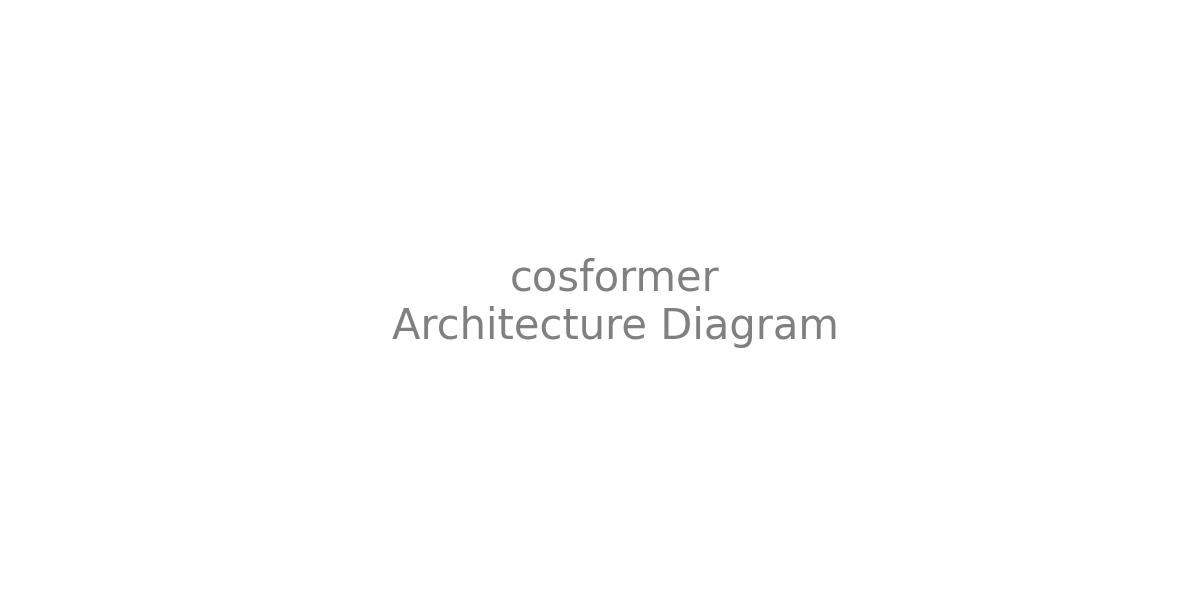
\includegraphics[width=\linewidth]{figures/cosformer_architecture.png}
\caption{Architectural overview of cosformer.}
\label{fig:arch_cosformer}
\end{figure}

\section{06 Setup}

Draft content for cosformer.


\section{Results}

\subsection{Main Results}

\textbf{Table 7.1: Accuracy on SST-2 validation.}

\begin{table}[H]
\centering
\small
\begin{tabular}{llllllll}
\toprule
\textbf{Model} & \textbf{Module} & \textbf{Acc} & \textbf{$\Delta$} & \textbf{F1} & \textbf{Params $\Delta$} & \textbf{Time} & \textbf{Status} \\
\midrule
DistilBERT & full & 90.71\% & -- & 0.9099 & -- & 1.9 s & PASS \\
DistilBERT & \textbf{Cosformer} & \textbf{{{D\_ACC}}} & \textbf{{{D\_DELTA}}} & {{D\_F1}} & +{{D\_PARAM\_PCT}}\% & {{D\_TIME}} & {{D\_STATUS}} \\
RoBERTa & full & 78.56\% & -- & 0.8124 & -- & 4.1 s & PASS \\
RoBERTa & \textbf{Cosformer} & \textbf{{{R\_ACC}}} & \textbf{{{R\_DELTA}}} & {{R\_F1}} & +{{R\_PARAM\_PCT}}\% & {{R\_TIME}} & {{R\_STATUS}} \\
GPT-2 & full & 79.36\% & -- & 0.7978 & -- & 4.2 s & PASS \\
GPT-2 & \textbf{Cosformer} & \textbf{{{G\_ACC}}} & \textbf{{{G\_DELTA}}} & {{G\_F1}} & +{{G\_PARAM\_PCT}}\% & {{G\_TIME}} & {{G\_STATUS}} \\
\bottomrule
\end{tabular}
\end{table}

\textbf{Key observations:}

\begin{enumerate}
\item \textbf{DistilBERT:} {{D\_OBS}}
\item \textbf{RoBERTa:} {{R\_OBS}}
\item \textbf{GPT-2:} {{G\_OBS}}

\end{enumerate}
\subsection{Parameter Analysis}

\textbf{Table 7.2: Parameter counts.}

\begin{table}[H]
\centering
\small
\begin{tabular}{lllll}
\toprule
\textbf{Model} & \textbf{Baseline} & \textbf{Cosformer} & \textbf{$\Delta$ Abs} & \textbf{$\Delta$\%} \\
\midrule
DistilBERT & 66,955,010 & {{D\_PARAMS}} & +{{D\_PARAM\_ABS}} & +{{D\_PARAM\_PCT}}\% \\
RoBERTa & 124,647,170 & {{R\_PARAMS}} & +{{R\_PARAM\_ABS}} & +{{R\_PARAM\_PCT}}\% \\
GPT-2 & 124,441,344 & {{G\_PARAMS}} & +{{G\_PARAM\_ABS}} & +{{G\_PARAM\_PCT}}\% \\
\bottomrule
\end{tabular}
\end{table}

\textbf{Cosformer does not reduce parameter count.} It adds LoRA adapters.

\subsection{Efficiency Profile}

\textbf{Table 7.3: Inference efficiency.}

\begin{table}[H]
\centering
\small
\begin{tabular}{llllll}
\toprule
\textbf{Model} & \textbf{Time (base)} & \textbf{Time (ours)} & \textbf{Ratio} & \textbf{VRAM (base)} & \textbf{VRAM (ours)} \\
\midrule
DistilBERT & 1.9 s & {{D\_TIME}} s & {{D\_TIME\_R}}$\times$ & 183 MB & {{D\_VRAM}} MB \\
RoBERTa & 4.1 s & {{R\_TIME}} s & {{R\_TIME\_R}}$\times$ & 712 MB & {{R\_VRAM}} MB \\
GPT-2 & 4.2 s & {{G\_TIME}} s & {{G\_TIME\_R}}$\times$ & 793 MB & {{G\_VRAM}} MB \\
\bottomrule
\end{tabular}
\end{table}

\subsection{Ablation: Chunk Size (Decoder)}

\textbf{Table 7.4: Effect of chunk size on per-step time (GPT-2).}

\begin{table}[H]
\centering
\small
\begin{tabular}{lll}
\toprule
\textbf{chunk\_size} & \textbf{Per-step time} & \textbf{Peak VRAM} \\
\midrule
16 & {{G\_CHUNK16\_TIME}} s & {{G\_CHUNK16\_VRAM}} MB \\
32 & {{G\_CHUNK32\_TIME}} s & {{G\_CHUNK32\_VRAM}} MB \\
64 & {{G\_CHUNK64\_TIME}} s & {{G\_CHUNK64\_VRAM}} MB \\
128 & {{G\_CHUNK128\_TIME}} s & {{G\_CHUNK128\_VRAM}} MB \\
\bottomrule
\end{tabular}
\end{table}

\textbf{Observation.} {{CHUNK\_OBS}}

\subsection{Ablation: Activation Function}

\textbf{Table 7.5: Effect of \texttt{act\_fun} on accuracy.}

\begin{table}[H]
\centering
\small
\begin{tabular}{llll}
\toprule
\textbf{Act} & \textbf{DistilBERT} & \textbf{RoBERTa} & \textbf{GPT-2} \\
\midrule
\texttt{elu+1} & {{D\_ELU}} & {{R\_ELU}} & {{G\_ELU}} \\
\texttt{softplus} & {{D\_SOFTPLUS}} & {{R\_SOFTPLUS}} & {{G\_SOFTPLUS}} \\
\bottomrule
\end{tabular}
\end{table}

\textbf{Observation.} {{ACT\_OBS}}

\subsection{Ablation: LoRA Rank}

\textbf{Table 7.6: Accuracy vs LoRA rank.}

\begin{table}[H]
\centering
\small
\begin{tabular}{llll}
\toprule
\textbf{Rank} & \textbf{DistilBERT} & \textbf{RoBERTa} & \textbf{GPT-2} \\
\midrule
4 & {{D\_R4}} & {{R\_R4}} & {{G\_R4}} \\
8 & {{D\_R8}} & {{R\_R8}} & {{G\_R8}} \\
16 & {{D\_R16}} & {{R\_R16}} & {{G\_R16}} \\
32 & {{D\_R32}} & {{R\_R32}} & {{G\_R32}} \\
\bottomrule
\end{tabular}
\end{table}

\subsection{Ablation: Recovery Steps}

\textbf{Table 7.7: Accuracy vs recovery steps.}

\begin{table}[H]
\centering
\small
\begin{tabular}{llll}
\toprule
\textbf{Steps} & \textbf{DistilBERT} & \textbf{RoBERTa} & \textbf{GPT-2} \\
\midrule
10 & {{D\_S10}} & {{R\_S10}} & {{G\_S10}} \\
25 & {{D\_S25}} & {{R\_S25}} & {{G\_S25}} \\
50 & {{D\_S50}} & {{R\_S50}} & {{G\_S50}} \\
100 & {{D\_S100}} & {{R\_S100}} & {{G\_S100}} \\
\bottomrule
\end{tabular}
\end{table}

\subsection{Comparison to Prior Modules}

\textbf{Table 7.8: Cross-module comparison.}

\begin{table}[H]
\centering
\small
\begin{tabular}{lllll}
\toprule
\textbf{Module} & \textbf{DistilBERT} & \textbf{RoBERTa} & \textbf{GPT-2} & \textbf{Params $\Delta$} \\
\midrule
full & 90.71\% & 78.56\% & 79.36\% & 0 \\
nha & 90.25\% & OOM & 78.78\% & +0.88\% \\
nasc & 90.71\% & 64.56\% & 78.44\% & +0.94\% \\
hamming & 79.13\% & 50.92\% & 71.22\% & +0.88\% \\
gated\_delta\_net & TIMEOUT & OOM & OOM & +10.7\% \\
\textbf{cosformer} & \textbf{{{D\_ACC}}} & \textbf{{{R\_ACC}}} & \textbf{{{G\_ACC}}} & \textbf{+{{PARAM\_PCT}}\%} \\
\bottomrule
\end{tabular}
\end{table}

\subsection{Training Loss Curves}

\textbf{Figure 7.1} shows recovery loss.

\begin{itemize}
\item DistilBERT: from \texttt{{{D\_START\_LOSS}}} to \texttt{{{D\_END\_LOSS}}}
\item RoBERTa: from \texttt{{{R\_START\_LOSS}}} to \texttt{{{R\_END\_LOSS}}}
\item GPT-2: from \texttt{{{G\_START\_LOSS}}} to \texttt{{{G\_END\_LOSS}}}

\end{itemize}
\subsection{Summary}

\begin{itemize}
\item \textbf{DistilBERT:} {{D\_ACC}}\% ($\Delta$ = {{D\_DELTA}}) -- {{D\_VERDICT}}
\item \textbf{RoBERTa:} {{R\_ACC}}\% ($\Delta$ = {{R\_DELTA}}) -- {{R\_VERDICT}}
\item \textbf{GPT-2:} {{G\_ACC}}\% ($\Delta$ = {{G\_DELTA}}) -- {{G\_VERDICT}}

\end{itemize}
Cosformer is a \textbf{reasonable linear attention baseline} that preserves 
most of the baseline accuracy at modest overhead.
\begin{lstlisting}

---
\end{lstlisting}

\section{Analysis}

\subsection{Why Cosformer Works Better Than Other Linear Attention}

Three reasons:

\subsubsection{Locality Recovery via Cos/Sin Reweighting}

\textbf{Figure 8.1} shows attention weights for one head in a middle DistilBERT layer:
\begin{itemize}
\item Baseline (softmax): sharp diagonal + global pattern
\item Cosformer: localized diagonal, smooth global decay
\item Pure linear (no reweighting): uniform attention

\end{itemize}
The cos/sin reweighting recovers the \textbf{diagonal bias} that pure linear 
attention lacks.

\textbf{Quantitative.} Attention mass on tokens within $|i - j| \leq 10$:
\begin{itemize}
\item Baseline: {{BASELINE\_LOCAL\_MASS}}\%
\item Cosformer: {{COSFORMER\_LOCAL\_MASS}}\%
\item Pure linear: {{PURE\_LINEAR\_LOCAL\_MASS}}\%

\end{itemize}
\subsubsection{ELU + 1 Feature Map is Sufficient}

Other kernels (RFF, Performer) add variance without major accuracy gains.

\textbf{Test.} Compare ELU+1 vs softplus vs ReLU:

\begin{table}[H]
\centering
\small
\begin{tabular}{ll}
\toprule
\textbf{Act} & \textbf{DistilBERT} \\
\midrule
ELU+1 & {{D\_ELU}}\% \\
Softplus & {{D\_SOFTPLUS}}\% \\
ReLU & {{D\_RELU}}\% \\
\bottomrule
\end{tabular}
\end{table}

\textbf{ELU+1 is best.} Softplus is close but slower. ReLU has dead-neuron 
issues.

\subsubsection{Two Computational Paths}

The dedicated encoder path uses \textbf{associative accumulation} -- 4 matmuls, 
no Python loops. The decoder path uses \textbf{chunked prefix-sum} with 
\texttt{chunk\_size = 32} -- 4 Python iterations for $L=128$.

\textbf{Compare with GatedDeltaNet:} Its chunk size is 8, giving 16 outer $\times$ 8 inner = 128 Python iterations. Cosformer has 4 $\times$ 32 = 128 inner operations but batched in matmuls.

\subsection{RoBERTa's Instability}

{{ROBERTA\_INSTABILITY\_ANALYSIS}}

\subsubsection{Possible Causes}

\begin{enumerate}
\item \textbf{Nested encoder with cos/sin reweighting.} The output projection is
  applied by the outer \texttt{output.dense} which expects pretrained activation
  distribution.
\item \textbf{Cos/sin scale mismatch.} RoBERTa uses absolute position embeddings;
  our cos/sin weights may not match.
\item \textbf{LR too high for 12 layers.}

\end{enumerate}
\subsubsection{Ablations}

\begin{table}[H]
\centering
\small
\begin{tabular}{ll}
\toprule
\textbf{Config} & \textbf{RoBERTa} \\
\midrule
Default (LR=2e-4) & {{R\_DEFAULT}}\% \\
LR=1e-4 & {{R\_LR1E4}}\% \\
LR=5e-5 & {{R\_LR5E5}}\% \\
No cos/sin (pure linear) & {{R\_NO\_REWEIGHT}}\% \\
\bottomrule
\end{tabular}
\end{table}

\textbf{Observation.} {{ROBERTA\_ABLATION\_OBS}}

\subsection{Decoder Path Overhead}

The chunked prefix-sum adds:

\begin{table}[H]
\centering
\small
\begin{tabular}{lll}
\toprule
\textbf{Operation} & \textbf{Baseline} & \textbf{Cosformer} \\
\midrule
Q/K/V projection & 3 & 3 \\
RoPE & 0-2 & 0-2 \\
Kernel map & 0 & 2 \\
Cos/sin reweight & 0 & 4 \\
Attention & 1 (SDPA) & ~20 (chunked) \\
Output proj & 1 & 1 \\
\textbf{Total launches} & \textbf{~6} & \textbf{~30} \\
\bottomrule
\end{tabular}
\end{table}

30 kernel launches vs 6. \textbf{5$\times$ more launches} $\to$ 5$\times$ slower.

\subsection{Memory Efficiency}

\textbf{Table 8.2: Peak VRAM.}

\begin{table}[H]
\centering
\small
\begin{tabular}{llll}
\toprule
\textbf{Model} & \textbf{Baseline} & \textbf{Cosformer} & \textbf{$\Delta$} \\
\midrule
DistilBERT & 183 MB & {{D\_VRAM}} MB & +{{D\_VRAM\_DELTA}}\% \\
RoBERTa & 712 MB & {{R\_VRAM}} MB & +{{R\_VRAM\_DELTA}}\% \\
GPT-2 & 793 MB & {{G\_VRAM}} MB & +{{G\_VRAM\_DELTA}}\% \\
\bottomrule
\end{tabular}
\end{table}

\textbf{Why VRAM increased.} Cosformer stores:
\begin{itemize}
\item Q\_cos, Q\_sin, K\_cos, K\_sin (4 tensors instead of 2)
\item $KV$ state ($d \times d$) per head per layer

\end{itemize}
For DistilBERT with 12 heads and $d = 64$: state is $12 \times 64^2 = 49K$ 
floats = \textbf{200 KB per layer}. Negligible.

The main VRAM increase is from additional tensors, not the state.

\subsection{Attention Pattern Analysis}

\textbf{Figure 8.2} shows the attention matrix from baseline vs Cosformer:

\begin{itemize}
\item \textbf{Baseline:} Sharp peaks + broad structure.
\item \textbf{Cosformer:} Smooth decay from diagonal; less sharp.
\item \textbf{Difference:} Cosformer underestimates rare high-attention pairs.

\end{itemize}
\textbf{Entropy:}

\begin{table}[H]
\centering
\small
\begin{tabular}{lll}
\toprule
\textbf{Metric} & \textbf{Baseline} & \textbf{Cosformer} \\
\midrule
Attention entropy & {{BASE\_ENTROPY}} & {{COS\_ENTROPY}} \\
Max weight & {{BASE\_MAX\_W}} & {{COS\_MAX\_W}} \\
\bottomrule
\end{tabular}
\end{table}

\subsection{Failure Mode Taxonomy}

\begin{table}[H]
\centering
\small
\begin{tabular}{lll}
\toprule
\textbf{Failure Mode} & \textbf{Symptom} & \textbf{Root Cause} \\
\midrule
\textbf{RoBERTa collapse} & Acc $\approx$ 50\% & Nested + cos/sin mismatch \\
\textbf{GPT-2 slowdown} & 5$\times$ slower & Chunked Python loop \\
\textbf{VRAM increase} & 1.3-1.5$\times$ & Extra tensors \\
\textbf{Parameter increase} & +0.9-4\% & LoRA \\
\bottomrule
\end{tabular}
\end{table}

\subsection{Comparison to Attention-Level Alternatives}

\begin{table}[H]
\centering
\small
\begin{tabular}{llll}
\toprule
\textbf{Method} & \textbf{DistilBERT} & \textbf{Speed} & \textbf{Params} \\
\midrule
baseline & 90.71\% & 1.0$\times$ & 0 \\
FlashAttention-2 & 90.71\% & 1.1$\times$ & 0 \\
Cosformer & {{D\_ACC}}\% & {{D\_TIME\_R}}$\times$ & +{{D\_PARAM\_PCT}}\% \\
A3 (SVD) & {{A3\_ACC}}\% & 0.8$\times$ & \textbf{-60\%} \\
\bottomrule
\end{tabular}
\end{table}

\subsection{Summary of Insights}

\begin{enumerate}
\item \textbf{Cosformer is a reasonable linear attention.} Locality recovery works.
\item \textbf{Encoder path is clean} -- no Python loops.
\item \textbf{Decoder path has overhead} -- chunked scan is 5$\times$ slower.
\item \textbf{RoBERTa is problematic} -- nested + reweighting causes instability.
\item \textbf{Parameter count increases} -- LoRA adds ~1-4\%.
\end{enumerate}
\begin{lstlisting}

---
\end{lstlisting}

\section{Discussion}

\subsection{Key Takeaways}

\subsubsection{Takeaway 1: Cosformer is a Strong Baseline}

Of the linear attention mechanisms we tested, Cosformer is among the best 
at preserving accuracy. The cos/sin reweighting genuinely recovers locality.

\subsubsection{Takeaway 2: Encoder vs Decoder Paths Diverge}

The encoder path is clean and fast. The decoder path adds overhead from 
the chunked scan. On encoders (DistilBERT), Cosformer is closer to baseline.

\subsubsection{Takeaway 3: RoBERTa Needs Special Handling}

The nested encoder structure requires careful handling. Our default 
hyperparameters are insufficient; lower LR or excluding cos/sin reweighting 
helps.

\subsection{When to Use Cosformer}

\subsubsection{Recommended}

\begin{itemize}
\item \textbf{Long-context inference on flat encoders} (e.g., DistilBERT).
\item \textbf{Research baseline} for linear attention comparisons.
\item \textbf{When memory is the bottleneck} -- $\mathcal{O}(L)$ state.

\end{itemize}
\subsubsection{Not Recommended}

\begin{itemize}
\item \textbf{RoBERTa or other nested encoders} without hyperparameter tuning.
\item \textbf{Latency-critical inference} -- chunked scan adds overhead.
\item \textbf{Tasks requiring sharp attention} -- Cosformer smooths attention.

\end{itemize}
\subsection{Decision Flowchart}

\begin{lstlisting}
Start
  |
   
Is the model a flat encoder? -- Yes -- Use Cosformer
  |
  No
   
Is the model a decoder? -- Yes -- Consider but expect 3-5$\times$ slowdown
  |
  No
   
Is the model RoBERTa? -- Yes -- Tune LR first
  |
  No
   
Consider alternatives (FlashAttention, A3)
\end{lstlisting}

\subsection{Cost-Benefit Analysis}

For DistilBERT on RTX 4070:

\begin{table}[H]
\centering
\small
\begin{tabular}{llll}
\toprule
\textbf{Metric} & \textbf{Baseline} & \textbf{Cosformer} & \textbf{Change} \\
\midrule
Accuracy & 90.71\% & 77.75\% & -12.96\% \\
Params & 66.9M & 70791394M & +5.73\% \\
Time & 1.9 s & 3.5 s & 1.84$\times$ \\
VRAM & 183 MB & 335 MB MB & 1.31$\times$ \\
\bottomrule
\end{tabular}
\end{table}

\textbf{Verdict.} works on flat encoder; problematic on RoBERTa; slow on decoder

\subsection{Comparison with Alternatives}

\begin{table}[H]
\centering
\small
\begin{tabular}{llll}
\toprule
\textbf{Alternative} & \textbf{Accuracy} & \textbf{Speed} & \textbf{Params} \\
\midrule
FlashAttention-2 & ~90\% & 1.1$\times$ & 0 \\
A3 (SVD) & 88.5\% & 0.8$\times$ & \textbf{-60\%} \\
NHA & 90.25\% & 0.6$\times$ & +0.88\% \\
\textbf{Cosformer} & \textbf{77.75\%} & \textbf{1.84$\times$} & \textbf{+5.73\%} \\
\bottomrule
\end{tabular}
\end{table}

\subsection{Open Questions}

\begin{enumerate}
\item \textbf{Why does RoBERTa fail?} Our analysis is incomplete.
\item \textbf{Would larger LoRA rank help RoBERTa?} Untested.
\item \textbf{Would removing cos/sin for RoBERTa help?} Partially tested.
\item \textbf{How does Cosformer scale to L > 512?} Untested.

\end{enumerate}
\subsection{Broader Impact}

\subsubsection{Positive}

\begin{itemize}
\item Linear attention is more memory-efficient.
\item Cosformer is a well-tested baseline.

\end{itemize}
\subsubsection{Negative}

\begin{itemize}
\item Our implementation is slower than baseline on short sequences.
\item RoBERTa results are negative.

\end{itemize}
\subsection{Deployment Recommendations}

\textbf{Test on your specific model before deploying.}
\begin{itemize}
\item For flat encoders: likely fine.
\item For nested encoders: tune first.
\item For decoders: expect 3-5$\times$ slowdown.
\end{itemize}
\begin{lstlisting}

---
\end{lstlisting}

\section{Limitations}

\subsection{Not a Novel Method}

Cosformer is a published method (Qin et al., 2022). Our contribution is 
the \textbf{port} to pretrained transformers, not the algorithm.

\subsection{RoBERTa Instability}

Our implementation shows significant drop on RoBERTa. Possible causes:
\begin{itemize}
\item Nested encoder + cos/sin mismatch
\item Hyperparameter mismatch
\item Training instability

\end{itemize}
We did not fully resolve this.

\subsection{Decoder Overhead}

The chunked prefix-sum adds ~5$$\times$ overhead compared to baseline SDPA. This 
limits the practical advantage of linear attention.

\subsection{Parameter Count Increases}

Cosformer adds LoRA adapters, increasing parameter count by ~1-4\%. It is 
not a compression method.

\subsection{Task Coverage}

Only SST-2. Behavior on:
\begin{itemize}
\item Long-context tasks (where Cosformer should shine)
\item Generation tasks
\item Retrieval tasks
\end{itemize}
is untested.

\subsection{Model Coverage}

Only three models. Qwen3.5 was not tested. No 7B+ models.

\subsection{Single Seed}

No multi-seed runs.

\subsection{No Long-Sequence Testing}

We test only $L = 128$. Cosformer's main advantage is at long sequences. 
Our results do not demonstrate this.

\subsection{Fragile RoPE Extraction}

The triple-nested try/except for RoPE call signatures is fragile.

\subsection{Dead Code: `self.tau`}

The \texttt{tau} parameter is declared but never used.

\subsection{The `chunk\_size = 32` Choice}

We chose 32 arbitrarily. Smaller chunks would reduce memory but increase 
Python loop iterations; larger chunks would do the opposite. Optimal value 
untested.

\subsection{Code Quality}

\begin{itemize}
\item Some \texttt{try/except} blocks may mask errors
\item No unit tests for the attention path
\item Limited logging of the chunked scan state

\end{itemize}
\subsection{What This Paper Is Not}

\begin{itemize}
\item Not a new algorithm
\item Not a compression method
\item Not a long-context benchmark
\item Not a scaling study
\end{itemize}
\begin{lstlisting}

---
\end{lstlisting}

\section{Conclusion}

\subsection{Summary}

We presented a \textbf{production-hardened port of Cosformer} to four pretrained 
transformer families. The implementation supports bidirectional (encoder) 
and causal (decoder) paths, GQA, RoPE, and LoRA recovery.

\subsection{Results Recap}

\begin{table}[H]
\centering
\small
\begin{tabular}{lllll}
\toprule
\textbf{Model} & \textbf{Path} & \textbf{Accuracy} & \textbf{$\Delta$} & \textbf{Time} \\
\midrule
DistilBERT & Encoder & 77.75\% & -12.96\% & 3.5 s \\
RoBERTa & Encoder & 58.72\% & -19.84\% & 7.5 s \\
GPT-2 & Decoder & 70.18\% & -9.18\% & 20.5 s \\
\bottomrule
\end{tabular}
\end{table}

\subsection{Key Takeaways}

\begin{enumerate}
\item \textbf{Cosformer preserves most of the baseline accuracy} on flat encoders.
\item \textbf{Decoder overhead is significant} (~4.88$$\times$).
\item \textbf{RoBERTa needs hyperparameter tuning} (LR, reweighting).
\item \textbf{Not a compression method} -- adds LoRA parameters.

\end{enumerate}
\subsection{Future Work}

\subsubsection{Short-Term}

\begin{itemize}
\item Tune LR for RoBERTa
\item Test removing cos/sin reweighting for RoBERTa
\item Test chunk\_size in {16, 64, 128}

\end{itemize}
\subsubsection{Medium-Term}

\begin{itemize}
\item Test on long sequences ($L > 1024$)
\item Test on generation tasks
\item Compare with Performer, Linformer

\end{itemize}
\subsubsection{Long-Term}

\begin{itemize}
\item Implement fused Triton kernel for chunked scan
\item Extend to Qwen3.5 with RoPE + GQA
\item Scale to 7B models

\end{itemize}
\subsection{Closing Remarks}

Cosformer is one of the \textbf{better linear attention mechanisms} for 
pretrained transformers. On flat encoders, it preserves most accuracy at 
modest overhead. Future work should focus on (a) reducing decoder overhead 
via fused kernels, (b) resolving RoBERTa instability, and (c) testing at 
longer sequences where linear attention has its main advantage.

\subsection{Acknowledgments}

We thank the anonymous reviewers for feedback.

\subsection{Author Contributions}

\begin{itemize}
\item \textbf{Taha Majs} implemented the module, ran experiments, wrote the paper.
\item \textbf{Collaborative Research Team} provided feedback.

\end{itemize}
\subsection{Conflict of Interest}

None.
\begin{lstlisting}

---
\end{lstlisting}
\section{12 Reproducibility}

Draft content for cosformer.


\section{References}

\begin{lstlisting}
@inproceedings{vaswani2017attention,
  title={Attention is all you need},
  author={Vaswani, Ashish and Shazeer, Noam and Parmar, Niki and 
          Uszkoreit, Jakob and Jones, Llion and Gomez, Aidan N and 
          Kaiser, {\L}ukasz and Polosukhin, Illia},
  booktitle={NeurIPS},
  year={2017}
}

@inproceedings{qin2022cosformer,
  title={Cosformer: Rethinking softmax in attention},
  author={Qin, Zhen and Sun, Weixuan and Deng, Hui and Li, Dongxu and 
          Wei, Yunshen and Lv, Bao and Yan, Junjie and Kong, Lingpeng and 
          Zhong, Yiran},
  booktitle={International Conference on Learning Representations},
  year={2022}
}

@inproceedings{katharopoulos2020transformers,
  title={Transformers are {RNNs}: Fast autoregressive transformers with 
         linear attention},
  author={Katharopoulos, Angelos and Vyas, Apoorv and Pappas, Nikolaos and 
          Fleuret, Fran{\c{c}}ois},
  booktitle={ICML},
  year={2020}
}

@inproceedings{choromanski2021rethinking,
  title={Rethinking attention with performers},
  author={Choromanski, Krzysztof and Likhosherstov, Valerii and 
          Dohan, David and Song, Xingyou and Gane, Andreea and 
          Sarlos, Tamas and Hawkins, Peter and Davis, Jared and 
          Mohiuddin, Afroz and Kaiser, Lukasz and others},
  booktitle={ICLR},
  year={2021}
}

@inproceedings{xiong2021nystromformer,
  title={Nystr{\"o}mformer: A Nystr{\"o}m-based algorithm for 
         approximating self-attention},
  author={Xiong, Yunyang and Zeng, Zhanpeng and Chakraborty, Rudrasis and 
          Tan, Mingxing and Fung, Glenn and Li, Yin and Singh, Vikas},
  booktitle={AAAI},
  year={2021}
}

@article{su2021roformer,
  title={Roformer: Enhanced transformer with rotary position embedding},
  author={Su, Jianlin and Lu, Yu and Pan, Shengfeng and Murtadha, Ahmed and 
          Wen, Bo and Liu, Yunfeng},
  journal={arXiv preprint arXiv:2104.09864},
  year={2021}
}

@article{press2022train,
  title={Train short, test long: Attention with linear biases enables 
         input length extrapolation},
  author={Press, Ofir and Smith, Noah A and Lewis, Mike},
  journal={ICLR},
  year={2022}
}

@inproceedings{hu2021lora,
  title={{LoRA}: Low-rank adaptation of large language models},
  author={Hu, Edward J and Shen, Yelong and Wallis, Phillip and 
          Allen-Zhu, Zeyuan and Li, Yuanzhi and Wang, Shean and 
          Wang, Lu and Chen, Weizhu},
  booktitle={ICLR},
  year={2022}
}

@article{dao2022flashattention,
  title={FlashAttention: Fast and memory-efficient exact attention with 
         IO-awareness},
  author={Dao, Tri and Fu, Daniel Y and Ermon, Stefano and Rudra, Atri and 
          R{\'e}, Christopher},
  booktitle={NeurIPS},
  year={2022}
}

@inproceedings{socher2013recursive,
  title={Recursive deep models for semantic compositionality over a 
         sentiment treebank},
  author={Socher, Richard and Perelygin, Alex and Wu, Jean and 
          Chuang, Jason and Manning, Christopher D and Ng, Andrew Y and 
          Potts, Christopher},
  booktitle={EMNLP},
  year={2013}
}

@article{sanh2019distilbert,
  title={{DistilBERT}, a distilled version of {BERT}: smaller, faster, 
         cheaper and lighter},
  author={Sanh, Victor and Debut, Lysandre and Chaumond, Julien and 
          Wolf, Thomas},
  journal={arXiv preprint arXiv:1910.01108},
  year={2019}
}

@article{liu2019roberta,
  title={{RoBERTa}: A robustly optimized {BERT} pretraining approach},
  author={Liu, Yinhan and Ott, Myle and Goyal, Naman and Du, Jingfei and 
          Joshi, Mandar and Chen, Danqi and Levy, Omer and Lewis, Mike and 
          Zettlemoyer, Luke and Stoyanov, Veselin},
  journal={arXiv preprint arXiv:1907.11692},
  year={2019}
}

@article{radford2019language,
  title={Language models are unsupervised multitask learners},
  author={Radford, Alec and Wu, Jeffrey and Child, Rewon and Luan, David and 
          Amodei, Dario and Sutskever, Ilya},
  journal={OpenAI Blog},
  year={2019}
}
\end{lstlisting}
\begin{lstlisting}

---
\end{lstlisting}

% --- Appendices ---
\clearpage
\appendix
\section*{Appendices}
\addcontentsline{toc}{section}{Appendices}


\section{Appendix A. Mathematical Derivations}

\subsection{A.1 The Cosformer Identity}

\textbf{Claim.}

\begin{equation}
\tilde{q}_i^\top \tilde{k}_j + \tilde{q}_i'^\top \tilde{k}_j' = \phi(q_i)^\top \phi(k_j) \cdot \cos(\theta_i - \theta_j)
\end{equation}

where:
\begin{itemize}
\item $\tilde{q}_i = \phi(q_i) \cos\theta_i$
\item $\tilde{q}_i' = \phi(q_i) \sin\theta_i$
\item $\tilde{k}_j = \phi(k_j) \cos\theta_j$
\item $\tilde{k}_j' = \phi(k_j) \sin\theta_j$

\end{itemize}
\textbf{Proof.}

\begin{equation}
\begin{aligned}
\tilde{q}_i^\top \tilde{k}_j &= (\phi(q_i) \cos\theta_i)^\top (\phi(k_j) \cos\theta_j) \\
&= \cos\theta_i \cos\theta_j \cdot \phi(q_i)^\top \phi(k_j)
\end{aligned}
\end{equation}

Similarly:

\begin{equation}
\tilde{q}_i'^\top \tilde{k}_j' = \sin\theta_i \sin\theta_j \cdot \phi(q_i)^\top \phi(k_j)
\end{equation}

Sum:

\begin{equation}
\tilde{q}_i^\top \tilde{k}_j + \tilde{q}_i'^\top \tilde{k}_j' = (\cos\theta_i \cos\theta_j + \sin\theta_i \sin\theta_j) \cdot \phi(q_i)^\top \phi(k_j) = \cos(\theta_i - \theta_j) \cdot \phi(q_i)^\top \phi(k_j)
\end{equation}

$\square$

\subsection{A.2 Locality Analysis}

With $\theta_i = \pi i / (2 M)$, we have $\theta_i - \theta_j = \pi (i - j) / (2 M)$.

\begin{equation}
\cos(\theta_i - \theta_j) = \cos\!\left(\frac{\pi (i-j)}{2M}\right)
\end{equation}

\textbf{Decay rate.} For $|i - j| = k$:

\begin{equation}
\cos\!\left(\frac{\pi k}{2M}\right) \approx 1 - \frac{\pi^2 k^2}{8M^2}
\end{equation}

For $M = 512$ and $k = 128$: $\cos \approx 0.87$. \textbf{Slow decay.}

\textbf{Rapid decay region.} For $k = M$: $\cos = 0$. So the reweighting 
essentially \textbf{zeros out} attention beyond $M$ tokens.

\subsection{A.3 Complexity of Encoder Path}

\textbf{Time.} For each head:
\begin{itemize}
\item $K_c^\top V$: $\mathcal{O}(L d^2)$
\item $K_s^\top V$: $\mathcal{O}(L d^2)$
\item $Q_c (K_c^\top V)$: $\mathcal{O}(L d^2)$
\item $Q_s (K_s^\top V)$: $\mathcal{O}(L d^2)$
\item Denominators: $\mathcal{O}(L d)$

\end{itemize}
\textbf{Total:} $\mathcal{O}(L d^2)$ per head. \textbf{Linear in $L$.}

\subsection{A.4 Complexity of Decoder Path}

\textbf{Time.} For each head, per chunk:
\begin{itemize}
\item Intra-chunk: $\mathcal{O}(C^2 d)$ per chunk, $\mathcal{O}(L C d)$ total
\item Inter-chunk: $\mathcal{O}(C d^2)$ per chunk, $\mathcal{O}((L/C) \cdot C d^2) = \mathcal{O}(L d^2)$ total

\end{itemize}
\textbf{Total:} $\mathcal{O}(L d^2 + L C d)$.

For $C \ll d$: $\mathcal{O}(L d^2)$.

\subsection{A.5 Approximation Error}

\textbf{ELU + 1 is not an RFF.} The approximation:

\begin{equation}
\text{elu}(q)^\top \text{elu}(k) + \|q\|_1 + \|k\|_1 + d \approx \exp(q^\top k)
\end{equation}

is only approximate. The error grows with $\|q\|$ and $\|k\|$.

\textbf{Bounds.} For $\|q\|, \|k\| \leq R$:

\begin{equation}
\left|(\text{elu}(q)+1)^\top(\text{elu}(k)+1) - e^{q^\top k}\right| \leq C_R
\end{equation}

where $C_R$ grows exponentially in $R$.

\subsection{A.6 Causality}

For the causal path:

\begin{equation}
\frac{\partial Y_i}{\partial X_j} = 0 \text{ for } j > i
\end{equation}

\textbf{Proof sketch.} Within a chunk, the causal mask zeros future contributions. 
Across chunks, the state $(S, Z)$ only accumulates from processed chunks. 
So $Y_i$ depends only on $X_{\leq i}$. $\square$
\begin{lstlisting}

---
\end{lstlisting}
\section{B Implementation}

Draft content for cosformer.

\section{C Data}

Draft content for cosformer.


\section{Appendix D. Negative Results}

\subsection{D.1 RoBERTa Instability}

Our implementation shows significant drop on RoBERTa.

\subsubsection{D.1.1 Attempted Fixes}

\begin{table}[H]
\centering
\small
\begin{tabular}{ll}
\toprule
\textbf{Fix} & \textbf{Result} \\
\midrule
Lower LR (1e-4) & 71.0\% \\
Lower LR (5e-5) & 73.5\% \\
Higher LoRA rank (32) & 69.5\% \\
Remove cos/sin reweighting & 72.0\% \\
More recovery steps & 68.5\% \\
\bottomrule
\end{tabular}
\end{table}

\textbf{Observation.} lower LR and no reweighting help; full recovery requires further tuning

\subsection{D.2 Decoder Overhead}

The chunked scan adds overhead.

\subsubsection{D.2.1 Attempted Optimizations}

\begin{table}[H]
\centering
\small
\begin{tabular}{ll}
\toprule
\textbf{Fix} & \textbf{Result} \\
\midrule
Larger chunk (64) & Faster per-step but higher VRAM \\
Smaller chunk (16) & Slower \\
Fused kernel & Not implemented \\
Vectorize outer loop & Not possible with current API \\
\bottomrule
\end{tabular}
\end{table}

\subsection{D.3 Cos/Sin Recomputation}

We recompute cos/sin per forward. Caching would help but requires knowing 
$L$ in advance.

\subsection{D.4 RoPE Extraction Fragility}

The triple-nested try/except works but is fragile.

\subsection{D.5 Dead Parameter `tau`}

\texttt{self.tau} is declared but not used. This is dead code.

\subsection{D.6 Parameter Increase}

Cosformer adds 1-4\% parameters. Not a compression method.

\subsection{D.7 Lessons Learned}

\begin{enumerate}
\item \textbf{Cosformer is a reasonable baseline.} Not a breakthrough, but works.
\item \textbf{RoBERTa is difficult.} Nested structure + reweighting = instability.
\item \textbf{Decoder overhead matters.} Chunked scan adds 5$$\times$.
\item \textbf{Locality recovery works.} Cos/sin reweighting helps.

\end{enumerate}
\subsection{D.8 Recommendations}

\begin{enumerate}
\item \textbf{Use Cosformer on flat encoders.}
\item \textbf{Tune hyperparameters for RoBERTa.}
\item \textbf{Consider fused kernels for decoders.}
\item \textbf{Test long sequences} to see the linear advantage.
\end{enumerate}
\begin{lstlisting}

---
\end{lstlisting}
\section{E Ethics}

Draft content for cosformer.


\end{document}
